\subsection{When the Continuum Hypothesis Haunts Probability Theory}

In foundational probability theory, you're not just asking whether a model converges—you’re asking whether it can even be \emph{defined} within a consistent mathematical universe. This is where the Continuum Hypothesis (CH) begins to matter.

\subsubsection{The Structure of \(\sigma\)-Algebras}

A probability space depends on a well-defined \(\sigma\)-algebra. The Lebesgue \(\sigma\)-algebra extends the Borel sets to include more “complicated” sets. But not all subsets of \(\mathbb{R}^n\) are measurable—especially when the Axiom of Choice or CH enters the scene.

If CH is true, it becomes easier to construct \emph{non-measurable sets} using well-orderings of \(\mathbb{R}\). This affects how large your \(\sigma\)-algebra can be, and whether a “universal” measure space even makes sense.

\subsubsection{The Existence of Non-Measurable Sets}

The CH influences the size and construction of pathological subsets of \(\mathbb{R}^n\), such as Vitali sets. These are:
\begin{itemize}
  \item Not Lebesgue measurable.
  \item Impossible to assign consistent volume or probability to.
  \item Constructed via transfinite selection—relying on assumptions like CH or the Axiom of Choice.
\end{itemize}

Such sets can break the basic assumptions of probability: they violate countable additivity, destroy well-defined expectations, and show that your probability model may be incomplete if you don’t restrict your domain carefully.

\subsubsection{Whether Functions Are Even Measurable}

In applied work, we assume functions are “nice”—continuous, integrable, measurable. But formally, a function \( f: \mathbb{R}^n \to \mathbb{R} \) is Lebesgue measurable only if the preimage of every Borel set is measurable.

If you define functions on all of \(\mathcal{P}(\mathbb{R}^n)\), you risk:
\begin{itemize}
  \item Including non-measurable domains.
  \item Constructing expectations that don’t exist.
  \item Assuming convergence where none is defined.
\end{itemize}

If CH is true, then all uncountable subsets of \(\mathbb{R}\) have size at most \(\aleph_1\), and your pathological functions follow specific rules. If CH is false, there might be “intermediate” cardinalities—functions and sets too big to tame, but too small to ignore.

\subsection*{Moral of the Story}

If you're:
\begin{itemize}
  \item Defining universal priors over continuous functions,
  \item Modeling with arbitrary subsets of \(\mathbb{R}^n\),
  \item Or proving results that claim to hold “for all measurable functions”—
\end{itemize}

\noindent Then the truth or falsity of CH can affect whether your model actually exists—or is just a Platonic fantasy conjured from unprovable axioms.

\subsection{Beyond Nyquist: Why the Vitali Set Is Like an Impossible Signal Sample}

To appreciate the implications of the Vitali set in the world of signal processing, imagine you're working with a digital audio signal. In practice, we sample a continuous waveform at regular intervals—say, 44,100 times per second for CD-quality audio. Each of these samples is a number we can store, process, and analyze.

Now suppose you had a “signal” defined by a Vitali set—where the values exist, but are chosen using the Axiom of Choice in a way that defies any measurable structure. What would that mean?

\begin{itemize}
  \item You couldn’t average its values over any interval—because there's no well-defined way to integrate or sum them.
  \item You couldn’t apply a Fourier transform—because there’s no consistent way to define energy or frequency content.
  \item You couldn’t even plot it meaningfully—because it resists being described in terms of measurable functions.
\end{itemize}

\textbf{Bottom line:} If Lebesgue measure is your ruler, then the Vitali set is a shape that shatters it. And in domains like signal processing, where measurement and structure are everything, that’s a serious philosophical curveball.


\begin{quote}
In signal processing terms, the Vitali set is like a waveform that has no frequency, no amplitude, no duration, and no structure—yet still “exists” on paper. It’s a theoretical object that breaks every tool you’d normally use to understand or manipulate signals.
\end{quote}


\textbf{In other words:} the success of Shannon's sampling theorem depends entirely on the assumption that the signal lives in a well-behaved mathematical universe—one where 

\begin{enumerate}
	\item integration makes sense, 
	\item Fourier transforms converge, and 
	\item the measure of a set is a meaningful quantity. 
\end{enumerate}

The moment you step outside that universe, things fall apart.





\begin{figure}[H]
\centering
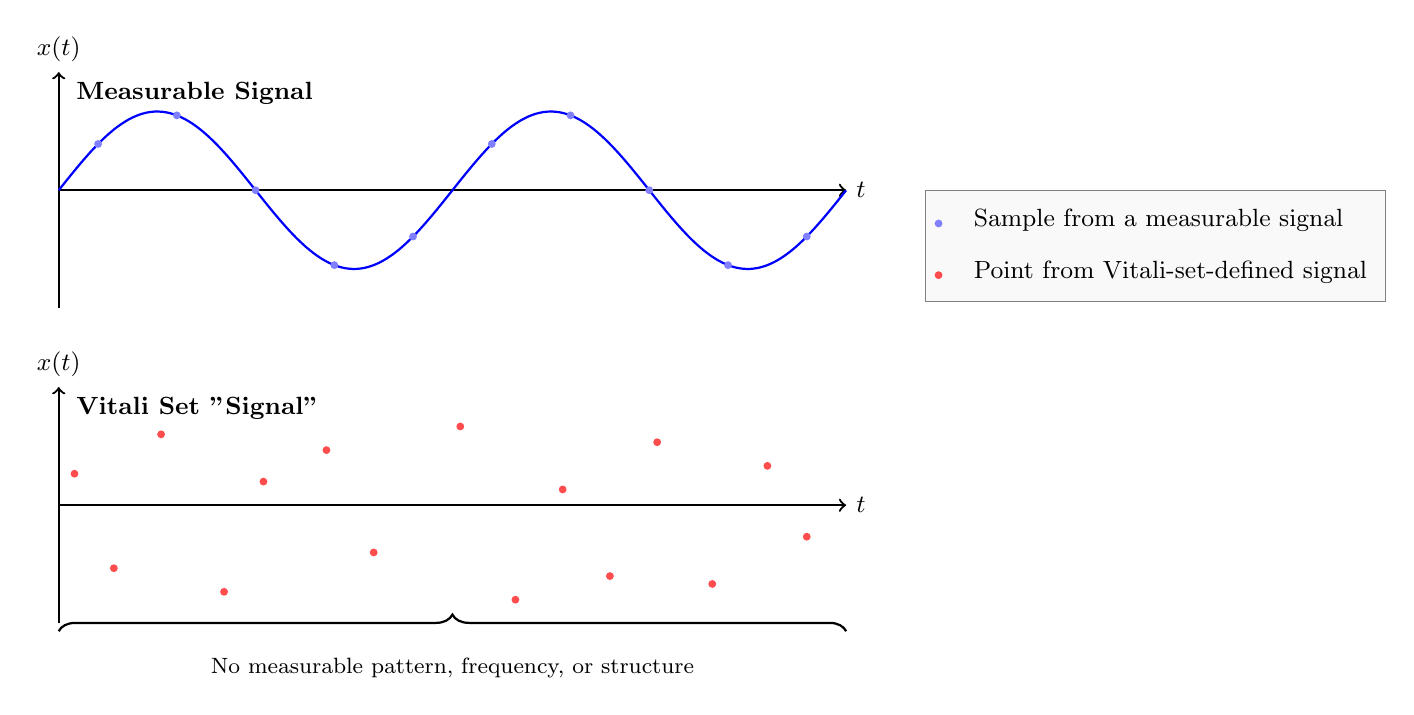
\begin{tikzpicture}[
    every node/.style={font=\small},
    axis/.style={->, thick},
    sample/.style={circle, fill=blue!50, inner sep=1pt},
    vitali/.style={circle, fill=red!70, inner sep=1pt},
    chaos/.style={draw=none, fill=red!20, minimum width=0.15cm, minimum height=0.6cm}
]

% Axis for measurable signal
\draw[axis] (0,0) -- (10,0) node[right] {\( t \)};
\draw[axis] (0,-1.5) -- (0,1.5) node[above] {\( x(t) \)};
\node[anchor=north west] at (0.1,1.5) {\textbf{Measurable Signal}};

% Draw sinusoid
\draw[thick, blue, domain=0:10, samples=100, smooth] plot(\x,{sin(2*pi*\x/5 r)});

% Sample points
\foreach \x in {0.5,1.5,...,9.5}
    \node[sample] at (\x,{sin(2*pi*\x/5 r)}) {};

% Axis for Vitali signal
\begin{scope}[yshift=-4cm]
\draw[axis] (0,0) -- (10,0) node[right] {\( t \)};
\draw[axis] (0,-1.5) -- (0,1.5) node[above] {\( x(t) \)};
\node[anchor=north west] at (0.1,1.5) {\textbf{Vitali Set "Signal"}};

% Chaos dots - unpredictable pattern
\foreach \x/\y in {
    0.2/0.4, 0.7/-0.8, 1.3/0.9, 2.1/-1.1, 2.6/0.3,
    3.4/0.7, 4.0/-0.6, 5.1/1.0, 5.8/-1.2, 6.4/0.2,
    7.0/-0.9, 7.6/0.8, 8.3/-1.0, 9.0/0.5, 9.5/-0.4
}
    \node[vitali] at (\x,\y) {};

% Annotate chaos zone
\draw[decorate,decoration={brace,amplitude=6pt}, thick] (0,-1.6) -- (10,-1.6) node[midway, below=6pt] {\footnotesize No measurable pattern, frequency, or structure};

\end{scope}

% Legend
\begin{scope}[shift={(11,0)}]
\matrix[draw=black!50, fill=gray!5, column sep=8pt, row sep=4pt, anchor=north west] {
  \node[sample] {}; & \node[anchor=west]{Sample from a measurable signal}; \\
  \node[vitali] {}; & \node[anchor=west]{Point from Vitali-set-defined signal}; \\
};
\end{scope}

\end{tikzpicture}
\caption{Top: a standard sinusoidal signal with well-defined samples. Bottom: a hypothetical signal defined by a Vitali set — unstructured, non-integrable, and incompatible with standard signal processing tools.}
\end{figure}


\vspace{1em}






